\section{Java Swing: Data Table}
\begin{frame}{Concepto de mantenedor}
\begin{block}{}
	%	\item[] crear():
	\begin{itemize}
		\item Interfaz de Usuario que permite administrar una base de datos mediante las operaciones de agregar, modificar y eliminar.
		\item Utilizados para  gestionar los registros almacenados en una base de datos, ya sea, una tabla de datos, un archivo u otra fuente de almacenamiento.
	\end{itemize}
\end{block}
\end{frame}

\begin{frame}{Concepto de mantenedor - Java}

	\begin{itemize}
\item Componente Java Swing cuya responsabilidad es la tabulaci\'on de datos.
\item Java provee de varios componentes swing para poder implementar de forma correcta mantenedores de fuentes de datos.
\item En general para esto se utiliza el componente JTable.
\item Se compone de Filas y Columnas.
\item Es posible seleccionar filas y extraer su valo mediante eventos de seleccion con perisfericos. Ejemplo: Mouse.
\end{itemize}
\end{frame}

\begin{frame}{Tips - Ocultamiento de Informaci\'on - Ejemplo.}
  \begin{figure}
    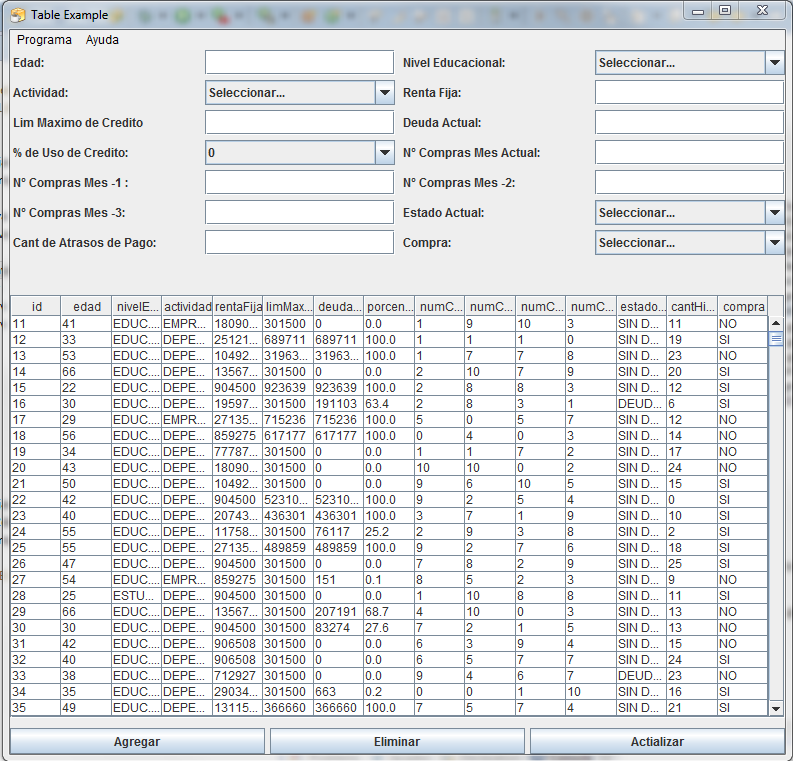
\includegraphics[scale=0.3]{figuras/DT.PNG}
  \end{figure}
\end{frame}

\begin{frame}{JTable: Instanciar Nueva}
\begin{block}{Ejemplo.}
	\lstinputlisting[language=Java,caption={},numbers=none]{resources/datatable/CrearDataTable.java}
\end{block}
\end{frame}

\begin{frame}{JTable: Agregar Regitro.}
\begin{block}{Ejemplo.}
	\lstinputlisting[language=Java,caption={},numbers=none]{resources/datatable/AddRow.java}
\end{block}
\end{frame}

\begin{frame}{JTable: Obtener Regitro.}
\begin{block}{Ejemplo.}
	\lstinputlisting[language=Java,caption={},numbers=none]{resources/datatable/GetRow.java}
\end{block}
\end{frame}

%\begin{frame}{Manejo de Excepciones - try, catch, finally}
%\begin{block}{Ejemplo.}
%\lstinputlisting[language=Java,caption={},numbers=none]{resources/excepciones/Finally.java}
%\end{block}
%\end{frame}
